% ===================================================================
%  Week 7 — Morphological Image Processing — Session 2
% ===================================================================
\documentclass[10pt,aspectratio=169]{beamer}
% ===================================================================
%  Shared Beamer preamble for "Practical Image Processing"
%  English slides. Compile with pdfLaTeX.
% ===================================================================

\usetheme{metropolis}
\usepackage[T1]{fontenc}
\usepackage[utf8]{inputenc}
\usepackage{lmodern}
\usepackage{listings}
\usepackage{tcolorbox}
\usepackage{fontawesome5}
\usepackage{booktabs}
\usepackage{amsmath,amssymb}
\usepackage{tikz}
\usepackage{pgfplots}
\pgfplotsset{compat=1.17}
\usetikzlibrary{arrows.meta,positioning,shapes.geometric,fit,backgrounds,matrix}
\tcbuselibrary{skins,breakable}

% ---- Palette --------------------------------------------------------
\definecolor{coursePrimary}{HTML}{1B4965}   % deep blue
\definecolor{courseAccent}{HTML}{E76F51}    % coral
\definecolor{courseGood}{HTML}{2A9D8F}      % teal
\definecolor{courseBad}{HTML}{C0392B}       % red
\definecolor{courseInfo}{HTML}{2980B9}      % blue
\definecolor{codeBg}{HTML}{F5F6FA}
\definecolor{codeKw}{HTML}{8E44AD}
\definecolor{codeStr}{HTML}{2A9D8F}
\definecolor{codeCom}{HTML}{7F8C8D}

\setbeamercolor{frametitle}{bg=coursePrimary}
\setbeamercolor{progress bar}{fg=courseAccent}
\setbeamercolor{alerted text}{fg=courseAccent}
\metroset{block=fill,sectionpage=progressbar,numbering=fraction}

% ---- Code listings (Python is built into listings) -----------------
\lstdefinestyle{course}{
  backgroundcolor=\color{codeBg},
  basicstyle=\ttfamily\scriptsize,
  keywordstyle=\color{codeKw}\bfseries,
  stringstyle=\color{codeStr},
  commentstyle=\color{codeCom}\itshape,
  numberstyle=\tiny\color{codeCom},
  numbers=left, numbersep=6pt,
  showstringspaces=false, breaklines=true, breakatwhitespace=true,
  tabsize=4, columns=fullflexible,
  frame=single, framesep=4pt, rulecolor=\color{gray!30},
  keepspaces=true, upquote=true, language=Python,
}
\lstset{style=course}
\lstdefinelanguage{bash}{
  keywords={cd,pip,python,venv,source,import}, sensitive=true,
  morecomment=[l]{\#}, morestring=[b]', morestring=[b]",
}

% ---- Reusable callout boxes ----------------------------------------
\newtcolorbox{goodbox}[1][Good practice]{colback=courseGood!8,colframe=courseGood,
  fonttitle=\bfseries,title={\faCheck~#1},boxrule=0.6pt,left=4pt,right=4pt,top=3pt,bottom=3pt}
\newtcolorbox{badbox}[1][Pitfall]{colback=courseBad!8,colframe=courseBad,
  fonttitle=\bfseries,title={\faTimes~#1},boxrule=0.6pt,left=4pt,right=4pt,top=3pt,bottom=3pt}
\newtcolorbox{infobox}[1][Note]{colback=courseInfo!8,colframe=courseInfo,
  fonttitle=\bfseries,title={\faInfoCircle~#1},boxrule=0.6pt,left=4pt,right=4pt,top=3pt,bottom=3pt}
\newtcolorbox{mathbox}[1][Math]{colback=coursePrimary!6,colframe=coursePrimary,
  fonttitle=\bfseries,title={\faCalculator~#1},boxrule=0.6pt,left=4pt,right=4pt,top=3pt,bottom=3pt}

\newcommand{\keyidea}[1]{\begin{alertblock}{Key idea}#1\end{alertblock}}
\newcommand{\term}[1]{\textbf{\color{coursePrimary}#1}}
\newcommand{\code}[1]{\lstinline[basicstyle=\ttfamily\small]|#1|}

% ---- A helper to draw a small pixel grid, cells shaded by value ----
% \pixelgrid{ {10,20,120,200,240}, {30,60,130,180,230}, ... }
\newcommand{\pixelgrid}[1]{%
  \begin{tikzpicture}[font=\scriptsize,scale=0.6]
    \foreach \row [count=\ry] in {#1} {
      \foreach \val [count=\cx] in \row {
        \draw[gray,fill=coursePrimary!8] (\cx,-\ry) rectangle ++(1,-1);
        \node at (\cx+0.5,-\ry-0.5) {\val};
      }
    }
  \end{tikzpicture}}


\title{Morphological Processing}
\subtitle{Week 7 — Session 2: Advanced operators \& the cleanup pipeline}
\author{Practical Image Processing}
\date{Lecture 7.2 \textbullet\ 60--70 min}

\begin{document}

\maketitle

\begin{frame}{Recap of Session 1}
  \begin{columns}[T]
    \begin{column}{0.58\textwidth}
      \begin{itemize}
        \item \term{Erosion} (fit) shrinks; \term{dilation} (hit) grows — set by a \term{structuring element}.
        \item \term{Opening} = erode$\to$dilate removes small bright specks (keeps size).
        \item \term{Closing} = dilate$\to$erode fills small gaps/holes (keeps size).
      \end{itemize}
    \end{column}
    \begin{column}{0.42\textwidth}
      \begin{alertblock}{Today}
        Compose these into \term{gradient}, \term{top-hat}, \term{black-hat}; go \term{grayscale}; remove lines; and build the DocScan cleanup pipeline + deliverable.
      \end{alertblock}
    \end{column}
  \end{columns}
\end{frame}

\begin{frame}{Roadmap}\tableofcontents\end{frame}

% ==================================================================
\section{Derived operators}
% ==================================================================

\begin{frame}{Morphological gradient, top-hat, black-hat}
  \begin{columns}[T]
    \begin{column}{0.4\textwidth}\begin{center}
      
\includegraphics[width=\linewidth]{../assets/gradient.png}\\{\scriptsize gradient = outline}
    \end{center}\end{column}
    \begin{column}{0.6\textwidth}
      \begin{itemize}
        \item \term{Gradient} $=$ dilation $-$ erosion $\rightarrow$ the object outline (thickness $\approx$ SE size).
        \item \term{Top-hat} $=$ image $-$ opening $\rightarrow$ small \emph{bright} details on a darker background.
        \item \term{Black-hat} $=$ closing $-$ image $\rightarrow$ small \emph{dark} details on a brighter background.
      \end{itemize}
    \end{column}
  \end{columns}
  \vspace{3pt}
  \begin{goodbox}
    Top-hat is a lighting fix: it isolates the digits from a slowly-varying background.
  \end{goodbox}
\end{frame}

\begin{frame}{Why top-hat corrects uneven lighting}
  \begin{itemize}
    \item Opening with a \emph{large} SE keeps only the smooth background (it erases small bright features).
    \item Subtracting that background — \code{image - opening} — leaves the small bright digits, flattened.
    \item Black-hat is the mirror image: it recovers small dark features sitting on a bright field.
  \end{itemize}
  \begin{mathbox}
    Top-hat$(f) = f - (f \circ B)$; \quad Black-hat$(f) = (f \bullet B) - f$. \ Choose $B$ larger than the details you want to keep.
  \end{mathbox}
\end{frame}

\begin{frame}{Gradient as an edge detector for shapes}
  \begin{center}
  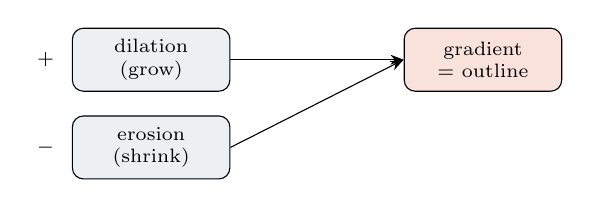
\begin{tikzpicture}[font=\scriptsize,>=Stealth,node distance=3mm and 8mm,
    b/.style={draw,rounded corners,fill=coursePrimary!8,minimum height=8mm,minimum width=20mm,align=center}]
    \node[b] (a){dilation\\(grow)};
    \node[b,below=of a] (c){erosion\\(shrink)};
    \node[b,right=22mm of a,fill=courseAccent!20] (g){gradient\\= outline};
    \draw[->](a.east)--(g.west);
    \draw[->](c.east)--(g.west);
    \node at (a.west) [left=1mm]{$+$};
    \node at (c.west) [left=1mm]{$-$};
  \end{tikzpicture}
  \end{center}
  \begin{itemize}
    \item The gradient is a band between the grown and shrunk shape — a clean, closed contour.
    \item Unlike a Sobel edge, it comes straight from a binary mask and is already one connected ring.
  \end{itemize}
\end{frame}

% ==================================================================
\section{Grayscale morphology}
% ==================================================================

\begin{frame}{Grayscale morphology}
  \begin{itemize}
    \item Morphology also works on grayscale: \term{erosion} $=$ local \emph{minimum}, \term{dilation} $=$ local \emph{maximum} under the SE.
    \item Opening/closing/top-hat all carry over — no thresholding required first.
    \item Top-hat on grayscale removes a smooth background gradient \emph{before} you threshold.
  \end{itemize}
  \begin{keyidea}{Morphology is not only for binary — on grayscale it is a nonlinear min/max filter that respects shape.}\end{keyidea}
\end{frame}

\begin{frame}{Grayscale erosion — worked example}
  Grayscale erosion replaces each pixel with the \emph{min} over a $1\times3$ window; dilation with the \emph{max}.
  \begin{center}
  \begin{tabular}{@{}rl@{}}
    input   & \pixelgrid{{40,90,90,20,90,90,40}}\\[6pt]
    erode (min) & \pixelgrid{{40,40,20,20,20,40,40}}\\[6pt]
    dilate (max) & \pixelgrid{{90,90,90,90,90,90,90}}\\
  \end{tabular}
  \end{center}
  \begin{itemize}
    \item The dark dip (20) spreads under erosion; bright plateaus spread under dilation.
    \item Top-hat here $=$ input $-$ opening would flag that narrow dark notch.
  \end{itemize}
\end{frame}

% ==================================================================
\section{Structuring-element design}
% ==================================================================

\begin{frame}{Structuring-element shapes}
  \begin{center}
  \begin{tabular}{@{}lll@{}}
    \toprule
    \textbf{Shape} & \textbf{When} & \textbf{Note} \\
    \midrule
    Rectangle & general cleanup & fast, blocky effect \\
    Ellipse & round objects & smoother, more natural \\
    Cross & thin connectors & minimal, gentle \\
    Line (h/v) & directional & remove/keep horizontal or vertical strokes \\
    \bottomrule
  \end{tabular}
  \end{center}
  \keyidea{A line SE can remove table lines while keeping text — the shape of the probe is a design choice.}
\end{frame}

\begin{frame}{Shape \& size both matter}
  \begin{itemize}
    \item A larger SE $=$ a stronger effect (removes bigger specks / fills bigger gaps) but more distortion.
    \item Shape matters: a vertical SE affects vertical strokes differently than a horizontal one.
    \item Rule: use the \emph{smallest} SE that fixes the defect — bigger erases real detail.
  \end{itemize}
  \begin{badbox}
    A too-large SE turns your digits into unrecognizable blobs. Tune the size on real data, not on a toy image.
  \end{badbox}
\end{frame}

\begin{frame}{Boundary extraction \& hole filling}
  \begin{columns}[T]
    \begin{column}{0.55\textwidth}
      \begin{itemize}
        \item \term{Boundary} $=$ image $-$ erosion (a thin inner outline; cf.\ the gradient which straddles the edge).
        \item \term{Hole filling}: fill enclosed dark regions inside a shape (a solid digit from a hollow one).
        \item Both compose from erosion/dilation — a small toolkit that builds many effects.
      \end{itemize}
    \end{column}
    \begin{column}{0.45\textwidth}
      \begin{center}
      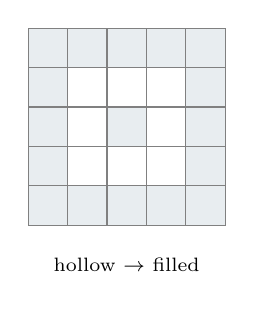
\begin{tikzpicture}[font=\scriptsize,scale=0.5]
        \foreach \x in {0,...,4}\foreach \y in {0,...,4}
          \draw[gray,fill=coursePrimary!10] (\x,-\y) rectangle ++(1,-1);
        \foreach \x in {1,2,3}\foreach \y in {1,2,3}
          \draw[gray,fill=white] (\x,-\y) rectangle ++(1,-1);
        \draw[gray,fill=coursePrimary!10] (2,-2) rectangle ++(1,-1);
        \node at (2.5,-6){\scriptsize hollow $\to$ filled};
      \end{tikzpicture}
      \end{center}
    \end{column}
  \end{columns}
\end{frame}

\begin{frame}{Skeletonization, thinning \& hit-or-miss}
  \begin{itemize}
    \item \term{Skeleton}: repeatedly thin a shape to a 1-pixel ``spine'' — its topological essence.
    \item Useful for character/stroke analysis and measuring connectivity.
    \item \term{Hit-or-miss} finds exact local patterns (corners, endpoints, junctions) with a foreground \emph{and} a background SE.
  \end{itemize}
  \begin{infobox}
    Skeletons are fragile to noise — clean with opening \emph{first}, or the spine sprouts spurious branches.
  \end{infobox}
\end{frame}

% ==================================================================
\section{The cleanup pipeline}
% ==================================================================

\begin{frame}{A morphology cleanup pipeline}
  \begin{center}
  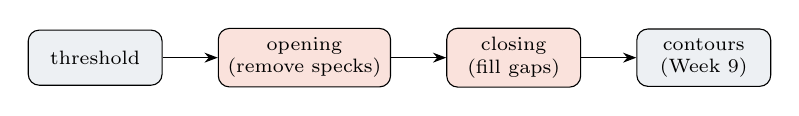
\begin{tikzpicture}[font=\scriptsize,>=Stealth,node distance=3mm and 7mm,
    b/.style={draw,rounded corners,fill=coursePrimary!8,minimum height=7mm,minimum width=17mm,align=center}]
    \node[b] (thr){threshold};
    \node[b,right=of thr,fill=courseAccent!20] (open){opening\\(remove specks)};
    \node[b,right=of open,fill=courseAccent!20] (close){closing\\(fill gaps)};
    \node[b,right=of close] (cc){contours\\(Week 9)};
    \draw[->](thr)--(open);\draw[->](open)--(close);\draw[->](close)--(cc);
  \end{tikzpicture}
  \end{center}
  \begin{itemize}
    \item Typical DocScan order: threshold $\rightarrow$ open (kill noise) $\rightarrow$ close (repair digits) $\rightarrow$ contours.
    \item Order matters: opening before closing avoids fusing a speck into a digit.
  \end{itemize}
\end{frame}

\begin{frame}{Removing lines, keeping text}
  \begin{itemize}
    \item A form has table/underline strokes you want gone but the text kept.
    \item Use a long \emph{horizontal} line SE with opening to isolate horizontal lines, then subtract them.
    \item A directional SE is a precise tool — it operates only on structures of a chosen orientation and length.
  \end{itemize}
  \begin{goodbox}
    For a scanned form (a DocScan case), this cleanly separates rules/boxes from the handwritten content.
  \end{goodbox}
\end{frame}

\begin{frame}[fragile]{Line removal in code}
\begin{lstlisting}[language=Python]
# isolate long horizontal rules, then subtract them
hks = cv2.getStructuringElement(cv2.MORPH_RECT, (25, 1))
lines = cv2.morphologyEx(binary, cv2.MORPH_OPEN, hks)
text_only = cv2.subtract(binary, lines)
\end{lstlisting}
  \begin{itemize}
    \item The $25\times1$ SE survives only along long horizontal runs — the table rules.
    \item Subtracting them leaves the digits; swap to $(1,25)$ for vertical rules.
  \end{itemize}
\end{frame}

\begin{frame}{Order of operations matters}
  \begin{itemize}
    \item \term{Open-then-close} vs \term{close-then-open} give \emph{different} results — the operations do not commute.
    \item Open first to kill specks, \emph{then} close: a leftover speck can otherwise be sealed into a digit.
    \item Top-hat/black-hat and gradient are also non-commuting compositions — always state the order.
  \end{itemize}
  \begin{badbox}
    Closing before opening can fuse a noise speck onto a stroke, creating a fake serif the OCR misreads.
  \end{badbox}
\end{frame}

\begin{frame}{Choosing the SE size for line removal}
  \begin{itemize}
    \item The horizontal SE length must exceed the \emph{thickest text stroke} but stay below the \emph{shortest rule} you want gone.
    \item Too short: text survives into the ``lines'' mask and gets subtracted away. Too long: short rules escape.
    \item Practical recipe: set length $\approx$ 1.5$\times$ the character width; verify on a real scan.
  \end{itemize}
  \begin{mathbox}
    A $(25,1)$ SE keeps runs $\ge 25$px wide horizontally — tune 25 to your scan resolution.
  \end{mathbox}
\end{frame}

\begin{frame}{Granulometry — measuring size by morphology}
  \begin{itemize}
    \item Open with SEs of increasing size and record how much foreground area disappears at each step.
    \item The drop at size $s$ counts objects roughly of size $s$ — a size \emph{distribution} without segmentation.
    \item A quick way to ask ``how big are my specks?'' before fixing the SE for opening.
  \end{itemize}
  \begin{infobox}
    Granulometry is morphology used as a \emph{measurement} tool, not just a cleanup tool.
  \end{infobox}
\end{frame}

\begin{frame}{Morphology vs blurring}
  \begin{itemize}
    \item Blurring averages (softens everything); morphology reasons about \emph{shape} (keeps edges hard).
    \item To remove specks from a \emph{binary} mask, opening beats a blur (which would gray it out).
    \item Use blur on grayscale/noise; use morphology on binary shapes.
  \end{itemize}
  \keyidea{Morphology is the right tool once you have a binary mask — it is shape surgery, not smoothing.}
\end{frame}

% ==================================================================
\section{In-class exercise}
% ==================================================================

\begin{frame}{\faPen~In-class exercise (10 min)}
  \begin{infobox}[Design the operator]
    Match each goal to a \emph{derived} operator and an SE, then say what you would subtract.
  \end{infobox}
  \begin{enumerate}
    \item Draw a one-pixel outline around every digit.
    \item Flatten a photo whose left side is darker than its right, before thresholding.
    \item Delete the underline printed beneath the meter reading, keeping the digits.
    \item Recover a faint dark serial number printed on a bright label.
  \end{enumerate}
\end{frame}

\begin{frame}{\faPen~Debrief}
  \begin{itemize}
    \item (1) \term{Gradient} (dilate $-$ erode) with a $3\times3$ SE.
    \item (2) \term{Top-hat} with a \emph{large} SE, then threshold the flattened result.
    \item (3) \term{Opening} with a long horizontal line SE, then \code{subtract}.
    \item (4) \term{Black-hat} with an SE larger than the characters.
  \end{itemize}
  \keyidea{Every derived operator is just erosion/dilation composed and subtracted — name the base, pick the SE, choose the sign.}
\end{frame}

% ==================================================================
\section{Wrap-up \& deliverable}
% ==================================================================

\begin{frame}{Derived operators — one-glance summary}
  \begin{center}
  \begin{tabular}{@{}lll@{}}
    \toprule
    \textbf{Operator} & \textbf{Definition} & \textbf{Use} \\
    \midrule
    Gradient  & dilation $-$ erosion & object outline \\
    Top-hat   & image $-$ opening    & small bright details, lighting fix \\
    Black-hat & closing $-$ image    & small dark details \\
    Boundary  & image $-$ erosion    & inner one-pixel edge \\
    \bottomrule
  \end{tabular}
  \end{center}
  \keyidea{Every row is erosion/dilation composed and subtracted. Learn the base pair and the rest are bookkeeping.}
\end{frame}

\begin{frame}[fragile]{All the operators in one call}
\begin{lstlisting}[language=Python]
k     = cv2.getStructuringElement(cv2.MORPH_ELLIPSE, (3, 3))
grad  = cv2.morphologyEx(binary, cv2.MORPH_GRADIENT, k)   # outline
top   = cv2.morphologyEx(gray,   cv2.MORPH_TOPHAT,   big_k) # lighting fix
black = cv2.morphologyEx(gray,   cv2.MORPH_BLACKHAT, big_k) # dark details
\end{lstlisting}
  \code{morphologyEx} covers open/close/gradient/top-hat/black-hat with one flag.
\end{frame}

\begin{frame}{Grayscale vs binary — which pipeline?}
  \begin{center}
  \begin{tabular}{@{}lll@{}}
    \toprule
    \textbf{You have} & \textbf{Do morphology\dots} & \textbf{Then} \\
    \midrule
    a clean scene, even light & after thresholding (binary) & open $\to$ close \\
    uneven lighting & \emph{before} thresholding (top-hat on gray) & then threshold \\
    faint dark marks & black-hat on gray & then threshold \\
    \bottomrule
  \end{tabular}
  \end{center}
  \begin{itemize}
    \item Grayscale morphology \emph{prepares} the image; binary morphology \emph{cleans} the mask.
    \item For a hard DocScan photo: top-hat, threshold, open, close — in that order.
  \end{itemize}
\end{frame}

\begin{frame}{What you should now be able to do}
  \begin{itemize}
    \item Apply gradient / top-hat / black-hat, and correct uneven lighting with top-hat.
    \item Explain grayscale morphology as a min/max filter; trace it on a row of values.
    \item Design a directional SE to remove lines while keeping text.
    \item Build a threshold $\rightarrow$ open $\rightarrow$ close cleanup pipeline for the digits.
  \end{itemize}
\end{frame}

\begin{frame}{This week's deliverable}
  \begin{alertblock}{Due before Week 8 (see \code{project/})}
    On a thresholded meter/plate (from Week 2):
    \begin{enumerate}
      \item Demonstrate erosion, dilation, opening, closing; explain each effect.
      \item Use opening to remove speckle noise and closing to repair broken digits.
      \item Apply top-hat to a photo with uneven lighting; compare to before.
      \item Use a directional line SE to strip a printed rule/underline while keeping the digits.
      \item DocScan milestone: produce a clean binary where each digit is a solid, separable blob.
    \end{enumerate}
  \end{alertblock}
\end{frame}

\begin{frame}[standout]
  Threshold makes it binary; morphology makes it clean.\\[4pt]
  \normalsize Compose erosion and dilation — gradient, top-hat, and a cleanup pipeline for the digits.
\end{frame}

\end{document}
